




\documentclass{beamer}
\usepackage[utf8]{inputenc}
\usepackage{url}
\usepackage{algorithm}
\usepackage{algpseudocode}
\usepackage{lmodern}
\usepackage{natbib}
\usepackage{tikz}
\usepackage{physics}
\usepackage{graphicx} % Allows including images
\usepackage{booktabs}
\usepackage{array}
\usepackage{listings}

\graphicspath{ {./images/} }
\usepackage{booktabs} % Allows the use of \toprule, \midrule and \bottomrule in tables
\usepackage{tikz}
%\usetikzlibrary{circuits.logic.US}
\usetikzlibrary{circuits.logic.US, positioning}

\usetikzlibrary{arrows.meta}

\usetikzlibrary{mindmap, trees, shadows, shapes, calc, fadings, positioning, decorations.pathreplacing, intersections, shapes, arrows}



% Style for Python-like code
\lstdefinestyle{python}{
  basicstyle=\ttfamily\scriptsize,
  keywordstyle=\color{blue},
  commentstyle=\color{gray},
  stringstyle=\color{red},
  showstringspaces=false,
  tabsize=2,
  breaklines=true
}


%\usetheme{Hannover}
%\usecolortheme{spruce}
% EPIC FAIL
\usetheme{default}
%\usecolortheme{beetle}
\usepackage{graphics}

\usepackage{color}
\definecolor{new_turquoise}{RGB}{40,151,158}%{251,190,94}
\setbeamercolor{title}{fg=new_turquoise}


%\usepackage[colorlinks=true, urlcolor=blue, linkcolor=red]{hyperref}


\makeatletter
\setbeamertemplate{frametitle}{
    \ifbeamercolorempty[bg]{frametitle}{}{\nointerlineskip}%
    \@tempdima=\textwidth%
    \advance\@tempdima by\beamer@leftmargin%
    \advance\@tempdima by\beamer@rightmargin%
    \vspace*{0.8cm} 
    %\hspace*{-3cm}
    %%%%%%%%%%%%% For example insert shift to right
    \begin{beamercolorbox}[sep=0.3cm,center,wd=\the\@tempdima]{frametitle}
        \usebeamerfont{frametitle}%
        \vbox{}\vskip-1ex%
        \if@tempswa\else\csname beamer@ftecenter\endcsname\fi%
        \strut\insertframetitle\strut\par%
        {%
            \ifx\insertframesubtitle\@empty%
            \else%
            {\usebeamerfont{framesubtitle}\usebeamercolor[fg]{framesubtitle}\insertframesubtitle\strut\par}%
            \fi
        }%
        \vskip-1ex%
        \if@tempswa\else\vskip-.3cm\fi% set inside beamercolorbox... evil here...
    \end{beamercolorbox}%
}
\makeatother

\setbeamercolor{frametitle}{fg=new_turquoise}
\setbeamertemplate{itemize item}{\color{new_turquoise}$\blacksquare$}
\setbeamertemplate{itemize subitem}{\color{new_turquoise}$\blacksquare$}


% --- ENUMERATE ITEMS ---
\setbeamertemplate{enumerate item}{\color{new_turquoise}\insertenumlabel}
\setbeamertemplate{enumerate subitem}{\color{new_turquoise}\insertsubenumlabel}

\setbeamertemplate{caption}{\raggedright\insertcaption\par}

% --- COLOR THE TABLE OF CONTENTS ENTRIES ---
\setbeamercolor{section in toc}{fg=new_turquoise}
\setbeamercolor{subsection in toc}{fg=new_turquoise}
\setbeamercolor{subsubsection in toc}{fg=new_turquoise}



% Set Beamer color themes
\setbeamercolor{block title}{fg=white, bg=new_turquoise}
\setbeamercolor{block body}{fg=black, bg=new_turquoise!10} % 10% opacity background


% Redefine theorem and corollary to use your color
% Set block colors (this is how Beamer themes work)
\setbeamercolor{block title}{fg=white, bg=new_turquoise}
\setbeamercolor{block body}{fg=black, bg=new_turquoise!10}

% Declare theorem environments AFTER setting colors
% \newtheorem{theorem}{Theorem}
%\newtheorem{corollary}[theorem]{Corollary}


\usebackgroundtemplate{
    
\includegraphics[width=\paperwidth,height=\paperheight]{figs/slide-title.jpg}
} 

\title{\fontsize{49}{7.2}{\bf Fundamental Algorithmic Techniques XII}}
%\author{JW}
\date{\color{new_turquoise}\today}
%S\titlegraphic{\includegraphics[width=2cm]{figs/jw.png}}

\begin{document}
\frame{\titlepage}
%% SLIDE 1 - INTRO TO THE TEAM
%%%%%%%%%%%%%%%%%%%%%%%%%%%%%%%%%%%%%%%%%%%%%%%%%%%%%

\usebackgroundtemplate{
    
\includegraphics[width=\paperwidth,height=\paperheight]{figs/slide-pages}
} 


\setbeamertemplate{subsection in toc}{
  \color{new_turquoise}$\blacksquare$\color{black}~~\inserttocsubsection
}


% Outline frame
\begin{frame}{Outline}
    \tableofcontents
\end{frame}





\section{Summary from functions theory}



\begin{frame}{Finite and Infinite Programming}

\begin{columns}[onlytextwidth]
\column{0.5\textwidth}
\textbf{Models of Computation}
\begin{itemize}
    \item \textbf{Circuits} → finite, fixed-size programs (exponential lengths...)
    \item \textbf{Automata} → handle infinite inputs/outputs, but limited to regular/simple problems
    \item \textbf{Turing Machine}\\
    \begin{itemize}
    \item One per problem
        \item Infinite, writable tape
        \item Finite set of inner states
        \item Transition function/table 
    \end{itemize}

    \item \textbf{Universal Turing Machine}\\
    Programmable computer!
\end{itemize}



\column{0.5\textwidth}
\small
\textbf{Turing-Complete Systems}

\begin{itemize}
    \item NAND-TM language
    \item RAM model (e.g., Python, C)
    \item Lambda calculus (e.g., Lisp, OCaml, Clojure)
    \item Cellular automata (e.g., Conway’s Game of Life)
\end{itemize}

\vfill
\begin{center}
\textcolor{new_turquoise}{\bf Church–Turing Thesis:} \\ 
\textit{A function on natural numbers is effectively computable} \\
$\Leftrightarrow$ \\
\textit{It is computable by a Turing machine.}
\end{center}
\end{columns}

\end{frame}


\begin{frame}{Turing Complete \& Computability }

\includegraphics[width=\linewidth]{Algos_figs/equicalentToTuring.png}

\textbf{
Let's have a closer look at computation types of classes! 
}

One can prove that {\bf infinitely many} functions:
$$\mathcal{F}: \{0,1\}^* \to {0,1}$$ are \textcolor{new_turquoise}{\bf uncomputable} by a Turing Machine.
\\
Well-known examples:
\begin{itemize}
    \item {\bf Halting Problem}:
    machine $M: \{0,1\}^* \to \{0, 1\}$, $\forall x \in \{0,1\}^*$, \\
    \begin{itemize}
        \item $\mathrm{Halt}(M, x) = 1$ if $M(x)$ halts
        \item else $\mathrm{Halt}(M, x) = 1$
    
    \end{itemize}
Proof sketch: function $\tilde M$ with infinite loop if $M(x)$ halts.
    \item {\bf Busy Beaver}:\\
    
    For a Turing Machine of n states: $M_n$, find longest max amount of steps before $M_n$ halts!
\end{itemize}
    
\end{frame}



\begin{frame}{Incomputability by Turing Machine}
One can prove that {\bf infinitely many} functions:
$$\mathcal{F}: \{0,1\}^* \to \{0,1\}$$ are \textcolor{new_turquoise}{\bf uncomputable} by a Turing Machine.

\bigskip
Well-known examples:
\begin{itemize}
    \item {\bf Halting Problem}: \\
    $\mathrm{Halt}(M, x) = 
    \begin{cases}
        1 & \text{if Turing machine } M \text{ halts on input } x, \\
        0 & \text{otherwise}.
    \end{cases}$ \\
    This function is uncomputable. \\
    %\textit{Proof sketch}: Assume a decider $H(M,x)$ exists; construct a machine $\tilde{M}$ that loops forever iff $H(M,M)=1$, leading to contradiction when run on itself.

    \item {\bf Busy Beaver}: \\
    For an $n$-state Turing machine $M_n$, find the maximum number of steps $M_n$ can run before halting (over all inputs and all such machines). Grows faster than any computable function!
\end{itemize}
\end{frame}


\section{Computational Classes}



\begin{frame}{Computational Complexity Classes — The Big Picture}
\centering
\footnotesize
\textbf{Decision problems} (answer: Yes/No)

\vspace{0.4cm}
\begin{tabular}{@{}lll@{}}
\toprule
\textbf{Class}       & \textbf{Meaning}                              & \textbf{Example}             \\ 
\midrule
\textbf{P}           & Solvable in poly-time                        & Sorting, shortest path       \\ 
\textbf{NP}          & Verifiable in poly-time                      & SAT, TSP (decision)          \\ 
\textbf{coNP}        & ``No'' answers verifiable in poly-time       & Formula validity             \\ 
\textbf{NP-complete} & In NP + NP-hard                              & 3-SAT, Clique                \\ 
\textbf{NP-hard}     & At least as hard as any NP problem           & Halting Problem, opt. TSP    \\ 
\textbf{Uncomputable} & Uncomputable as seen above & Halting Problem, Busy Beaver, ... \\
\bottomrule
\end{tabular}

\end{frame}



\begin{frame}{NP-hard, and NP-complete}
\begin{columns}[onlytextwidth]
\column{0.5\textwidth}
\centering
\includegraphics[width=0.9\linewidth]{Algos_figs/NPNPhard.png} \\


\smallskip
\footnotesize
Relationships among P, NP, NP-complete, and NP-hard classes.\\ 
One assumes $P\ne NP$ but it is unproven.

\column{0.5\textwidth}
\begin{itemize}
    \item \textbf{NP-hard}: A problem $\Pi$ is NP-hard if a polynomial-time algorithm for $\Pi$ would imply a polynomial-time algorithm for every problem in NP.
    \item \textbf{NP-complete}: A problem that is both NP-hard and an element of NP.
\end{itemize}
\footnotesize
\vspace{0.5cm}
\end{columns}
\end{frame}





\begin{frame}{SAT, 3SAT, and NP-Completeness}

\centering
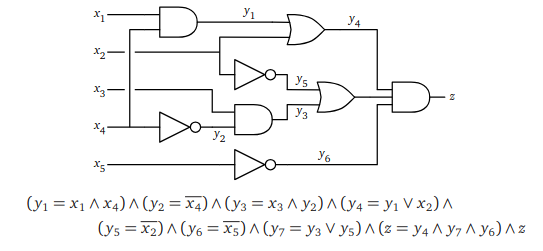
\includegraphics[width=0.6\linewidth]{Algos_figs/circuittobooleanexpression.png}

\medskip
\footnotesize
Every Boolean circuit $\mathcal{C}: \{0,1\}^n \to \{0,1\}$ can be converted in $\mathcal{O}(n)$ time to an equivalent Boolean formula or satisfiability problem {\bf SAT}.\\
\bigskip
\bigskip

\scriptsize
\begin{block}{Circuit-SAT $\leq_p$ SAT}
The \textbf{Cook–Levin Theorem} shows: \\
Any NP computation can be encoded as a Boolean circuit → then as a formula. \\
Thus, \textbf{SAT is NP-hard}.
\end{block}



\end{frame}



\begin{frame}{SAT, 3SAT, and NP-Completeness}

\scriptsize

\begin{block}{SAT $\in$ NP}
SAT serves as a polynomial-size certificate → verifiable in poly-time.

\medskip
$\Rightarrow$ \textbf{SAT is NP-complete}.
\end{block}

\begin{block}{3SAT}
Restrict SAT to CNF formulas with \textbf{exactly 3 literals per clause}. \\
\textbf{3SAT is also NP-complete} (via polynomial reduction from SAT). \\
Widely used in hardness proofs.
\end{block}

\bigskip
\bigskip
\bigskip

\footnotesize
Karp (1972) showed 21 problems (including 3SAT, Clique, Vertex Cover) are NP-complete via reductions from SAT.

\end{frame}





\begin{frame}{$P \neq NP$ versus $P = NP$?}
\begin{columns}[onlytextwidth]
\column{0.5\textwidth}
\centering
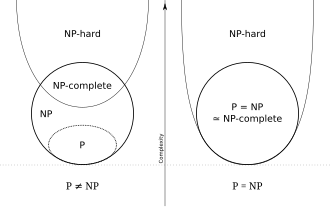
\includegraphics[width=0.95\linewidth]{Algos_figs/P_np_np-complete_np-hard.svg.png}

\smallskip
\tiny
Relationships among P, NP, NP-complete, and NP-hard classes. \\
The standard assumption is \(P \neq NP\), but this remains unproven.

\column{0.5\textwidth}
\smallskip
\textbf{If \(P = NP\):}
\begin{itemize}
    \item Every efficiently verifiable solution can also be efficiently found.
    \item \textbf{Breakdown} of modern cryptography (e.g., RSA, ECC).
    \item \textbf{Revolution} in optimization, logistics, scheduling.
    \item \textbf{Transformative advances} in AI, machine learning, and automated reasoning.
    \item Many currently intractable problems become tractable.
\end{itemize}

\textbf{Status:} unsolved question 
\end{columns}
%https://diffstudy.com/difference-between-np-hard-and-np/
\end{frame}

\section{Shannon Entropy}

% ==================== SLIDE 1 ====================
\begin{frame}{Shannon Entropy — Information is Surprise}
\small
\centering
\textbf{How much \textcolor{new_turquoise}{information} does a random variable carry?}

\vspace{.1cm}
\[
H(X) = -\sum p_i \log_2 p_i \quad \text{(in bits per symbol)}
\]

\vspace{0.1cm}
\begin{tabular}{ccc}
Coin & $P(\text{Heads})$ & $H(X)$ \\ \hline
Fair         & 50\%  & \textbf{1.00 bit}  ← maximum uncertainty \\
99\% heads   & 99\%  & $\approx 0.08$ bit ← boring \\
1\% heads    & 1\%   & $\approx 6.6$ bits ← shocking when it lands!
\end{tabular} \\

$$H(X)_{Fair} \approx 1.0 \quad VS \quad H(X)_{99\%} = 0.08!!! $$


\vspace{.1cm}
\large
\textcolor{new_turquoise}{\textbf{Entropy = average surprise}} \\
\textbf{1 bit} = one perfect yes/no question

\vspace{0.5cm}
\small
English text: $H \approx 1$ bit/character  
→ 1 MB of text can be compressed to ~125 KB (in theory)
\end{frame}






% ==================== SLIDE 2 ====================
\begin{frame}{The Source Coding Theorem — The Hard Limit}
\small
\textbf{Shannon’s Source Coding Theorem (1948)}:

For a source with entropy $H(X)$ bits/symbol:

\begin{itemize}
    \item You \textbf{cannot} compress below $H(X)$ bits/symbol on average
    \item You \textbf{can} get arbitrarily close — but only for \textcolor{red}{very long} messages
    \item In practice: English $\approx 1$ bit/character → best possible compression $\approx 12.5\%$ of raw text
\end{itemize}

\vspace{.5cm}
\small
\textbf{Consequences for LLMs training:} \\


\vspace{0.2cm}
\small
Shannon Entropy  versus Cross entropy loss: \\
$H(P)=\sum_i p_i \cdot \mathrm{log}(p_i)$ versus 
$H(P, Q)=\sum_i p_i \cdot \mathrm{log}(q_i)$ 

\begin{itemize}
    \item Modern LLMs reach ~7–8 bits/token → within ~10–20\% of the theoretical limit.
    \item Limit for cross entropy loss around 1 (as $Q \to P$). 

\end{itemize}
\end{frame}


% ==================== SLIDE 1 — KOLMOGOROV ====================
\section{Kolmogorov Complexity}

\begin{frame}{Kolmogorov Complexity }

\vspace{.1cm}
\textbf{Kolmogorov}: ``What is the shortest program that outputs this exact string?''

\bigskip 

\textcolor{new_turquoise}{\textbf{K(x) = length of shortest program that prints x and halts}}\\

\medskip
→ The \textbf{true} information content of one object (not a distribution)\\

\medskip
{\textbf{Uncomputable}} ($\sim$ because of Halting Problem)\\
%\tiny
\scriptsize

\vspace{.5cm}
{\bf Examples:}
\begin{itemize}
    \item simple objects: $K(x)=\mathrm{log}(n)$
    \item random objects: $K(x) = n +\mathrm{O}(\mathrm{log}(n))$ (expensive!)
    \item $x = 2^m$: $K(x) = \mathrm{log}(m) $ (finite code $f(z)=2^z$ + description of m)
\end{itemize}
\smallskip
\begin{tabular}{c|c|c}
String & Length & K(x) in bits \\ \hline
\texttt{01010101…} (1 million times) & 8 MB & $\approx 100$ bits \\
\texttt{π = 3.14159…} (first million digits) & 8 MB & $\approx 200$ KB \\
\texttt{War and Peace} & 3 MB & $\approx 4–5$ MB \\
Random noise (1 MB) & 1 MB & $\approx 8\cdot10^6$ bits (incompress!)
\end{tabular}

\end{frame}





\section{Solomonoff Induction}
\begin{frame}{Solomonoff - Kolmogorov  Complexity}

{\bf Definition}:\\
task $T: \{0,1\}^* \to \{0,1\}$. 
$$K(T) = min_{p\in T} \mid p \mid, $$
   where $\mid p \mid$ is length of the code. \\
\medskip
\medskip
{\bf Theorem}:\\
Consider two Universal Turing machines M, N (Kolmogorov):
$$K_N-C \leq K_M \leq K_N + C .$$
With C a constant.  Complexity is equivalent for two  programming languages, up to the compiler differences (that become negligeable when $K_M$ large).


  
\bigskip 

Nb of lines that can be written by humans is small compared to learning machines.

\end{frame}




\begin{frame}{Solomonoff Induction \& Completeness}
\scriptsize
\textbf{1. Bayesian model selection}  
Given data $D$ and a theory $T$, Bayes’ rule gives the posterior:
\[
\mathbb{P}[T \mid D] = 
\frac{\mathbb{P}[D \mid T]\, \mathbb{P}[T]}
{\mathbb{P}[D \mid T]\, \mathbb{P}[T] + \sum_{A \neq T} \mathbb{P}[D \mid A]\, \mathbb{P}[A]}
\]

\medskip
\textbf{2. Predicting future data $F$}  
The optimal predictive distribution marginalizes over all theories:
\[
\mathbb{P}[F \mid D] = \mathbb{E}_T\!\big[ \mathbb{P}[F \mid T, D] \big] 
= \sum_T \mathbb{P}[F \mid T, D]\, \mathbb{P}[T \mid D]
\]

\medskip
\textbf{3. Solomonoff completeness (error bound)}  
Let $T^*$ be the {\it perfect theory}. The \textit{total expected prediction error} of Solomonoff induction is bounded by the \textbf{Kolmogorov complexity} of $T^*$ (simplified: learning works!!!):
\[
\sum_{t=1}^\infty \mathbb{E}\big[ \, |\mathbb{P}(F_t \mid D_{<t}) - \mathbb{P}_{\text{true}}(F_t \mid D_{<t})| \, \big] \;\lesssim\; K(T^*)
\]
%\[
%\sum_{t=1}^\infty \mathbb{E}\!\left[ D_{\mathrm{KL}}\!\big( \mu(\cdot|x_{<t}) \,\|\, M(\cdot|x_{<t}) \big) \right] 
%\leq \frac{K(T^*)}{\ln 2}
%\]

%where $M$ is the universal Solomonoff prior and $K(T^*)$ is the length (in bits) of the shortest program describing $T^*$.

\smallskip
\textcolor{new_turquoise}{
\textbf{LLMs are gradient descent trying to be Solomonoff induction with 175 billion parameters.}
}
%https://www.youtube.com/watch?v=_kzwJ7Z-rfQ

\end{frame}



\end{document}
